\chapter{Thermal effects}

In this chapter, we put a focus on thermal effects. For low temperatures we
find the entropy to be negative for separations $L/R \gtrsim 0.04$. The
numerical results suggest that the entropy is still negative for smaller
separations and vanishes for $L/R\to0$. In the high temperature limit the free
energy becomes independent of the particular properties of the metal in the
Drude model. This enables us to study this limit for perfect reflectors as well
as Drude mirrors. We compare our numerical results with expressions obtained by
PFA and various suggested expansion of the free energy for small separations.
In the last section, we investigate thermal effects for perfect mirrors at
intermediate separations.


\section{Low temperatures}
\label{section_thermal_low_temp}

The expansion of the free energy for low temperatures is given by
\begin{equation}
\label{eq:temp_lt_approx}
\mathcal{F}(T) \approx a+bT^4.
\end{equation}
The coefficient $a$ corresponds to the free energy at $T=0$
\begin{equation}
a \equiv \mathcal{F}(T=0),
\end{equation}
and $b$ to the low temperature entropy divided by $-4T^3$:
\begin{equation}
S = -\frac{\partial\mathcal{F}}{\partial T} = -4bT^3 \\ \Rightarrow b = -\frac{S}{4T^3}
\end{equation}
We have derived analytical expressions for the free energy for small separations
\eqref{eq:pfa_T0} using the PFA approximation in chapter \ref{chapter_pfa}, and for large separations
\eqref{eq:ld_F_LT} using the dipole approximation in chapter \ref{chapter_ld}.
In order to obtain $a$ and $b$ for arbitrary separations, the free
energy is computed numerically for 20 temperatures in the range $T=0.05\dots0.25$. The
coefficients $a$ and $b$ are then obtained using linear regression in the
variable $T^4$.

\begin{figure}
  \begin{minipage}[b]{.5\linewidth}
  \centering
  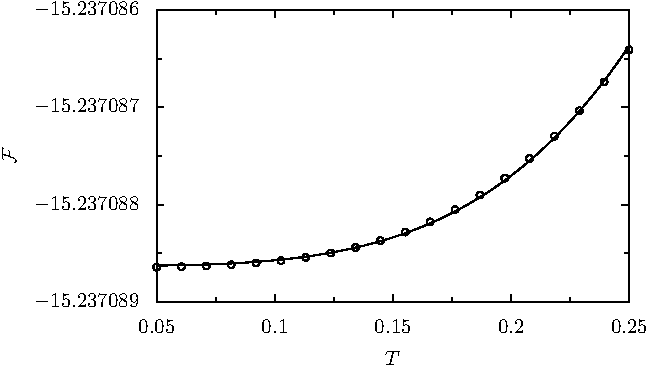
\includegraphics[scale=0.7]{plots/lowT_fit/fits/fit_0_052718.pdf}
  \subcaption{$L/R = 0.052718$}
  \end{minipage}
  \begin{minipage}[b]{.5\linewidth}
  \centering
  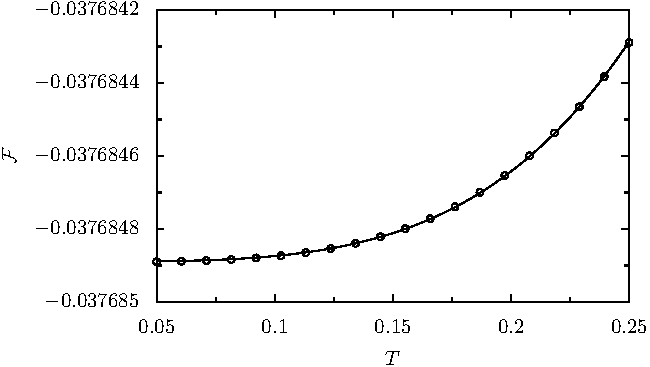
\includegraphics[scale=0.7]{plots/lowT_fit/fits/fit_1_001202.pdf}
  \subcaption{$L/R = 1.001202$}
  \end{minipage}

  \caption{Low temperature fits for the free energy using $\mathcal{F}\approx
  a+bT^4$ for a) $L/R\approx0.05$ and b) $L/R\approx1$. The points correspond
  to numerical data, the solid lines to \eqref{eq:temp_lt_approx}
  with parameters $a$ and $b$ obtained using linear regression.}
  \label{fig:temp_lowT_fits}
\end{figure}

In order to obtain meaningful results it is important to discuss the
reliability and the accuracy of the fit parameters $a$ and $b$. On the one
hand, the points $P_i=(T_i,\mathcal{F}(T_i))$ used for the fit must not be
computed for too high temperatures, because \eqref{eq:temp_lt_approx} is only
valid for small temperatures. On the other hand, for low temperatures the free
energy hardly changes. For the numerical computation we used
$\epsilon_p=10^{-10}$ and $\lmax=\max\left(25, \lceil \eta \, L/R
\rceil\right)$, where $\eta = 6.2$. For separations $L/R \ge 1$ this yields a
very high accuracy of about $10^{-8}$--$10^{-9}$. However, for smaller
separations the accuracy is limited by the choice of $\lmax$ and is in the
order of $10^{-4}$--$10^{-5}$. Fig. \ref{fig:temp_lowT_fits} shows two fits
for $L/R\approx0.05$ and $L/R\approx1.0$. The agreement of the numerical
points and the fit functions are in both cases good. However, the deviation of
the fits from the numerical points becomes stronger for smaller separations.

The change of the free energy in Fig. \ref{fig:temp_lowT_fits} a) is smaller
than the accuracy of the free energy. Nevertheless, the following two examples
show that this causes no numerical problems. For $L/R=0.1$ and $L/R=0.07$ we
compare the parameters $a$ and $b$ obtained using $\epsilon_p = 10^{-10}$,
$\eta=6.2$, and a much preciser computation using $\eta=12.4$.
\begin{center}
\begin{tabular}{|c|c|c|c|c|}
\hline
        & \multicolumn{2}{c|}{$L/R=0.1$} & \multicolumn{2}{c|}{$L/R=0.07$} \\
\hline
$\eta$  & $6.2$       & $12.4$ & $6.2$ & $12.4$ \\
\hline
$\lmax$ & $62$        & $124$  & $89$  & $178$ \\
\hline
$a$     & $-4.200585$ & $-4.200709$    & $-8.613663$ & $-8.613869$ \\
\hline
$b$     & $6.279343\cdot10^{-4}$ & $6.279350\cdot10^{-4}$ & $6.094080\cdot10^{-4}$ & $6.094146\cdot10^{-4}$ \\
\hline
\end{tabular}
\end{center}
Both parameters $a$ and $b$ hardly change and we see that $\eta=6.2$ yields
satisfactory results. The reason for this is as following: The accuracy is not limited
by $\epsilon_p$, but by the choice of $\eta$. For increasing values of $\eta$ the computed free energy
converges monotonic to the exact free energy. The convergence hardly depends on
the temperature (cf. Fig \ref{fig:convergence_lmax}) and thus the points used for the fits are shifted in the order of the
accuracy. Therefore, the accuracy of $a$ and $b$ is in the order of the free energy.

In Fig. \ref{fig:temp_lowT} we plot the free energy and the entropy for $T=0$
versus the separation. For small separations the free energy conincides with
the approximation obtained by the PFA, and for large separations the free energy
coincides with the approximation obtained in the large--distance limit. The
entropy for low temperatures is negative for separations $0.036 \le L/R \le
10$. For large separations the parameter $b$ is given by (cf. \eqref{eq:ld_F_LT})
\begin{equation}
b = \frac{1}{240\pi} \left(\frac{R}{\mathcal{L}}\right)^3 = \frac{1}{240\pi \, (1+L/R)^3}.
\end{equation}
Thus the entropy is negative and tends to zero for $L/R\to\infty$. The entropy
reaches a minimum at $L/R \approx 0.104$ and $S/(4T^3) \approx
-6.28\cdot10^{-4}$. In the PFA approximation the Casimir entropy is always
positive. As the PFA is a good approximation for small separations, it is
plausible that the entropy tends to zero for $L/R\to0$.

\begin{figure}
\begin{minipage}[b]{.5\linewidth}
\centering
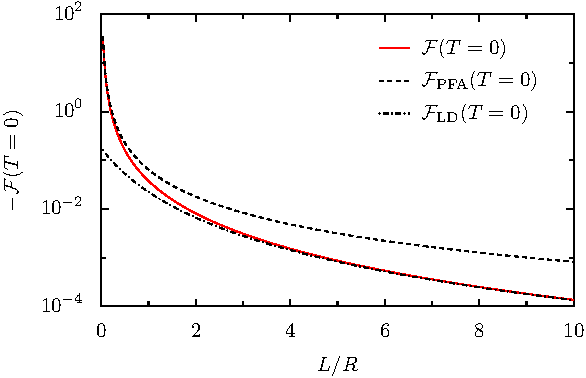
\includegraphics[scale=0.78]{plots/lowT_fit/F0.pdf}
\subcaption{free energy}
\end{minipage}
\begin{minipage}[b]{.5\linewidth}
\centering
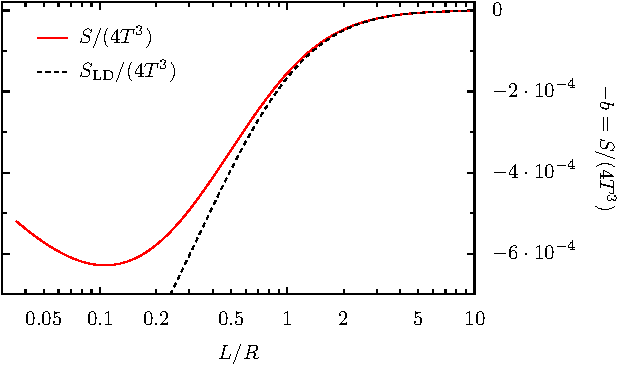
\includegraphics[scale=0.78]{plots/lowT_fit/S0.pdf}
\subcaption{entropy}
\end{minipage}

\caption{We plot a) the free energy and b) the low temperature entropy versus
the separation of plane and sphere. For small separations the free energy
coincides with the PFA result, for large separations the free energy coincides
with the large--distance limit. For large separations the entropy tends to
zero, for smaller separations it decreases and reaches a minimum at $L/R
\approx 0.104$ and $S/(4T^3) \approx 6.28\cdot10^{-4}$.}
\label{fig:temp_lowT}
\end{figure}


\section{High temperatures}
\label{section_thermal_hi_temp}
\newcommand{\lnmu}{\log\,\mu}

For perfect reflectors the free energy is a universal function depending only
on the temperature $T$ and the ratio $x=L/R$. In this section, we study the
high temperature limit of the Casimir effect. In this limit the free energy is
dominated by the $n=0$ term and higher Matsubara frequencies may be
neglected. The matrix elements of the scattering operator are given by the
analytical expressions \eqref{eq:scattering_ps_conclusion_xi0_EE} and
\eqref{eq:scattering_ps_conclusion_xi0_MM}. These expressions are also for
Drude metals independent of the particular properties of the metal. For this
reason, the free energy only depends on temperature and separation in the high temperature
limit. This, however, is not true for the plasma model, because the Fresnel
coefficient $r_\TE$ still depends on $\omega_P$ and $\kappa$ for $\xi\to0$.
Moreover, the numerical evaluation of the free energy in the high temperature
limit is considerable simpler than for low and intermediate temperatures. This
enables us to study notably smaller separations. In this section, we will mainly
follow Ref. \cite{PhysRevA.85.052501}.

\begin{figure}
\begin{center}
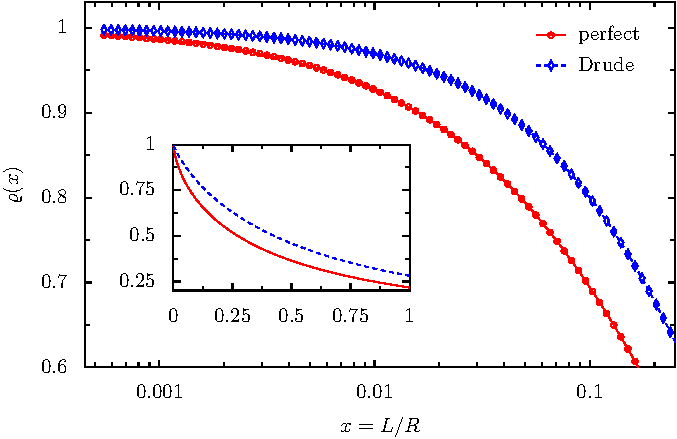
\includegraphics[scale=1]{plots/hiT/rho_vs_lnx.pdf}
\end{center}

\caption{The ratio $\varrho$ of the exact free energy and the PFA approximation
in the Drude model and for perfect reflectors versus the separation $L/R$. The
inset shows $\varrho$ for separations up to $L/R=1$.}
\label{fig:temp_hi_rho}
\end{figure}


In the high temperature limit we may only consider the $n=0$ term and the free
energy becomes
\begin{equation}
\mathcal{F}^\text{HT}\left(T, L/R\right) = \frac{T}{2\pi} \sum_m^\prime \mathcal{D}^{(m)}(nT=0).
\end{equation}
As the free energy depends linear on the temperature, the entropy becomes
constant. The scattering matrices $\mathcal{D}^{(m)}$ depend on the ratio
$x=L/R$ and we are lead to define
\begin{equation}
\label{eq:temp_hi_def_phi}
\mathcal{F}^\text{HT}(T, L/R) = \frac{T}{2\pi} \Phi(L/R), \\ \Phi(L/R) \equiv \sum_m^\prime \mathcal{D}^{(m)}(nT=0).
\end{equation}
The function $\Phi$ is universal in the Drude model and for perfect reflectors,
however, both functions are not identical. We will distinguish both functions
using superscripts ``D'' for Drude model and ``P'' for perfect reflectors.

With \eqref{eq:pfa_HT} and \eqref{eq:pfa_HT_drude} the ratio of the exact
result and the PFA approximation is given by
\begin{equation}
\varrho^{\text{D},\text{P}}(x) \equiv \frac{\mathcal{F}^\text{HT}}{\mathcal{F}^\text{HT}_\text{PFA}} = -\frac{x\,\Phi^{\text{D},\text{P}}}{C^{\text{D},\text{P}}}, \\
C^\text{D} \equiv \frac{\xi(3)}{8}, \sep C^\text{P} \equiv \frac{\xi(3)}{4},
\end{equation}
where we have used the approximated PFA results. The discrepancy between the
ratio $\varrho$ for Drude and perfect mirrors is caused by the different behaviour
of $r_\TE$ for $\xi\to0$. In Fig. \ref{fig:temp_hi_rho} the ratio $\varrho$ versus
the separation $x=L/R$ is plotted. The ratio $\varrho$ tends to one for separations
$x\to0$.
For a given ratio $L/R$ the accuracy of the
PFA is better for the Drude model than for perfect reflectors. The accuracy of the leftmost
points $L/R\approx5.53\cdot10^{-4}$ is only $\varrho^\text{P}\approx0.9914$ for perfect
reflectors, but $\varrho^\text{D}\approx0.9979$ for Drude mirrors.
In Fig. \ref{fig_temp_hiT_phi_beta} a) we plot the universal function $\Phi(x)$ for the
Drude model and perfect reflectors. For perfect reflectors $-\Phi$ is greater
than for Drude mirrors. The ratio $\Phi^\text{P}/\Phi^\text{D}$ tends to 2 for
$L/R\to0$ and reaches a value of $3/2$ for $L/R\to\infty$ \cite{ThermalCasimirEffect}.
The numerical results were obtained using $\epsilon_p=5\cdot10^{-9}$ and
$\eta=8$, for the leftmost point $\lmax=14465$ was used for the calculation.

\begin{figure}
  \begin{minipage}[b]{.5\linewidth}
  \centering
  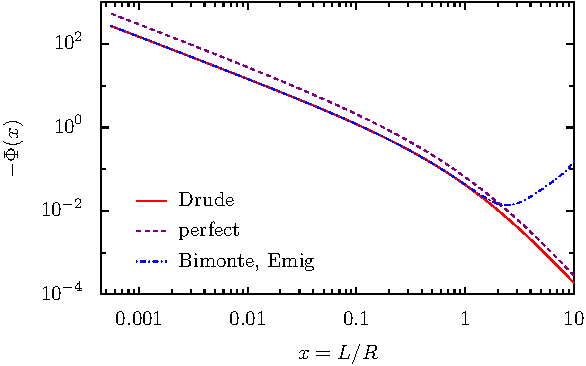
\includegraphics[scale=0.79]{plots/hiT/hiT_perf_drude_emig_bimonte.pdf}
  \subcaption{high temperature free energy}
  \end{minipage}%
  \begin{minipage}[b]{.5\linewidth}
  \centering
  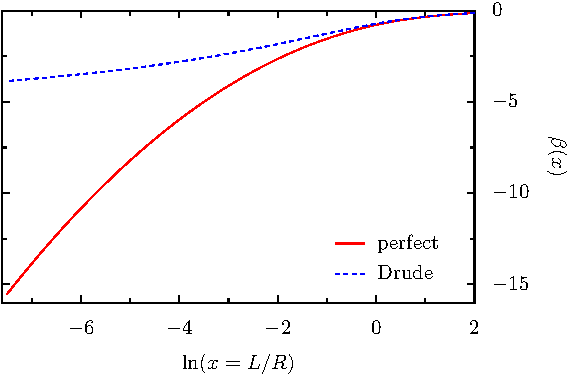
\includegraphics[scale=0.79]{plots/hiT/hiT_3_beta_vs_lnx.pdf}
  \subcaption{additive correction to PFA}
  \end{minipage}
  \ \\
  \begin{minipage}[b]{.5\linewidth}
  \centering
  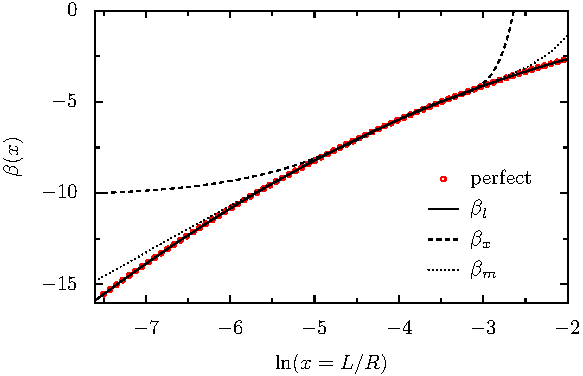
\includegraphics[scale=0.79]{plots/hiT/hiT_4_beta_vs_lnx_perfect_fits.pdf}
  \subcaption{$\beta^\text{P}$ and trial functions}
  \end{minipage}%
  \begin{minipage}[b]{.5\linewidth}
  \centering
  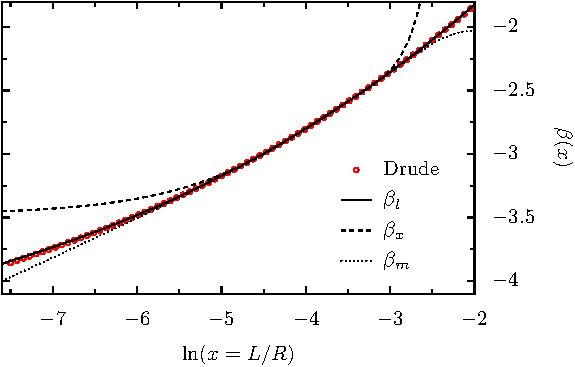
\includegraphics[scale=0.79]{plots/hiT/hiT_6_beta_vs_lnx_drude_fit.pdf}
  \subcaption{$\beta^\text{D}$ and trial functions}
  \end{minipage}
  \ \\
  \caption{In a) we show the universal function $-\Phi(x)$ versus the separation $x=L/R$
  for the Drude model and for the model of perfect reflectors. The function $\Phi = 2\pi\mathcal{F}/T$ is
  proportional to the free energy.
  We also plot an expansion of $\Phi$
  for small separations derived by \textsc{Bimonte} and \textsc{Emig} \cite{PhysRevLett.109.160403}.
  In b) the additive correction $\beta$ to PFA is plotted
  for Drude mirrors and perfect reflectors in the range $-7.5 \le \log(L/R) \le 2$.
  We plot the function $\beta(x)$ together with the trial functions $\beta_l$, $\beta_x$ and $\beta_m$
  in c) for perfect reflectors and in d) for the Drude model.}

  \label{fig_temp_hiT_phi_beta}
\end{figure}

Following an idea of \textsc{Canaguier--Durand}, \textsc{Ingold}, \textsc{Jackel} et al. \cite{PhysRevA.85.052501},
we express the ratio $\varrho$ by
\begin{equation}
\beta^{\text{D},\text{P}}(x) \equiv \frac{\varrho^{\text{D}, \text{P}}(x)-1}{x},
\end{equation}
where $\beta^{\text{D},\text{P}}$ corresponds to an additive correction to PFA
\begin{equation}
\Phi^{\text{D},\text{P}}(x) = -C^{\text{D},\text{P}} \left(\frac{1}{x} + \beta^{\text{D},\text{P}}(x)\right).
\end{equation}
The functions $\beta^{\text{D},\text{P}}$ are depicted in Fig.
\ref{fig_temp_hiT_phi_beta} b) in the range $-7.5 \le L/R \le 2$. For large
separations the functions $\beta^\text{D}$ and $\beta^\text{P}$ coincide.
For the function $\beta$ we consider following trial functions:
\begin{align}
\beta_l(x) &= a_0 + a_1 \log x + a_2 \log^2 x + a_3 \log^3 x \\
\beta_x(x) &= b_0 + b_1 x + b_2 x^2 + b_3 x^3 \\
\beta_m(x) &= c_0 + c_1 \log x + c_2 x + c_3 x^2
\end{align}
The first function is a polynomial in the variable $\log x$, the second
function is a polynomial in $x$, and the last function is a mixed form that
results from the assumption that the force in the high temperature limit can be expressed as a Laurent series
in $x$. The parameters are obtained from the numerical
results using fits in the interval $\log x \in [-5, -3]$. In total, 27 points
were used for the fits. The function $\beta$ and the trial functions
$\beta_l$, $\beta_x$ and $\beta_m$ are depicted in Fig. \ref{fig_temp_hiT_phi_beta}
for c) perfect reflectors and d) for the Drude model.
The fit parameters for the trial functions for perfect reflectors are
\begin{align}
\nonumber
a_0^\text{P} &= -0.824834,  & a_1^\text{P} &= 0.545277,   & a_2^\text{P} &= -0.181948,    & a_3^\text{P} &= 0.000932, \\
\nonumber
b_0^\text{P} &= -10.187688, & b_1^\text{P} &= 364.692140, & b_2^\text{P} &= -8750.230389, & b_3^\text{P} &= 78825.984591, \\
\nonumber
c_0^\text{P} &=  5.222405,  & c_1^\text{P} &= 2.634690,   & c_2^\text{P} &= -40.064506,   & c_3^\text{P} &= 226.000366,
\end{align}
and for the Drude model
\begin{align}
\nonumber
a_0^\text{D} &= -0.474404,  & a_1^\text{D} &= 0.780873,   & a_2^\text{D} &=  0.056193,    & a_3^\text{D} &= 0.001597, \\
\nonumber
b_0^\text{D} &= -3.478220,  & b_1^\text{D} &= 53.680980,  & b_2^\text{D} &= -1075.234122, & b_3^\text{D} &= 9158.452023, \\
\nonumber
c_0^\text{D} &= -1.715240,  & c_1^\text{D} &= 0.301137,   & c_2^\text{D} &=  7.149318,    & c_3^\text{D} &= -37.457065.
\end{align}
The trial functions $\beta_x$ and $\beta_m$ behave similar for perfect reflectors
and in the Drude model. The numerical results show that $\beta_x$ coincides
with $\beta$ only in a small window. The function $\beta_m$ agrees with $\beta$
in a broader domain, but it also differs significantly from $\beta$ for small
separations. Therefore $\beta$ cannot be expressed as a polynomial in $x$, and
the assumption that the force can be expressed as a Laurent series in $x$ is
not valid in general. The trial function $\beta_l$ behaves different for perfect
reflectors and in the Drude model. For perfect reflectors $\beta_l$ is in
perfect agreement with $\beta$ for small separations. For the Drude model
$\beta_l$ is still in good agreement, however, the trial function differs from
$\beta$ noticeably for small separations. So, the numerical results suggest
that $\beta$ can be approximated by a polynomial in $\log x$ for perfect
reflectors, but not in the Drude model. Our results are in agreement with
\cite{PhysRevA.85.052501}, however, as we arrive at smaller separations, we can
also show that $\beta_l$ differes from $\beta$ for the Drude model.

\begin{figure}
    \begin{center}
    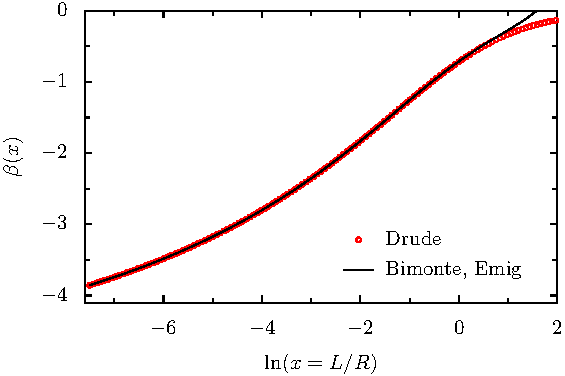
\includegraphics[scale=1]{plots/hiT/hiT_7_beta_vs_lnx_drude_bimonte.pdf}
    \end{center}

    \caption{Additive correction $\beta$ to the PFA and the approximation given by \textsc{Bimonte} and \textsc{Emig} \cite{PhysRevLett.109.160403}.
    Both functions are in perfect agreement for small separations.}
    \label{temp_hiT_emigbimonte}
\end{figure}

Moreover, we want to compare our numerical results with an analytical expression
of the free energy derived by \textsc{Bimonte} and \textsc{Emig} for Drude
metals \cite{PhysRevLett.109.160403}. This
expression is supposed to be valid for small separations in the high
temperature limit. The function $\Phi$ is given by
\begin{align}
\nonumber
\Phi_\text{BE}^\text{D}(x) = \frac{1}{2} \, \Bigg[& -\frac{\xi(3)}{2\mu^2} + \frac{\lnmu}{12} + \frac{1}{8} - \gamma_0 - \frac{7\mu^2}{2880} - \frac{31\mu^4}{725760} \\
\label{eq:temp_hiT_emigbimonte}
&\log\left(\gamma_1-\lnmu\right) + \frac{-\gamma_2+\lnmu}{-\gamma_1+\lnmu} \frac{\mu^2}{6} - \frac{\gamma_3-\gamma_4\lnmu+\log^2\mu}{(-\gamma_1+\lnmu)^2} \frac{\mu^4}{180} + \mathcal{O}\left(\mu^6\right)\Bigg],
\end{align}
where
\begin{equation}
\mu \equiv \ln\left(1+x+\sqrt{x(2+x)}\right).
\end{equation}
The constants $\gamma_0 = 0.174897$, $\gamma_1 = 0.1270362$, $\gamma_2 =
1.35369$, $\gamma_3 = 1.59409$ and $\gamma_4 = 2.51153$ are given by integrals,
but \textsc{Bimonte} and \textsc{Emig} give only an expression for the integral of $\gamma_0$.
Fig. \ref{temp_hiT_emigbimonte} shows $\beta^\text{D}$ and the function $\beta_\text{BE}^\text{D}$ obtained from
$\Phi_\text{BE}^\text{D}$. Both functions are for small separations in perfect
agreement. In Fig. \ref{fig_temp_hiT_phi_beta} a) the free energy in terms of $\Phi$
is plotted with the approximation \eqref{eq:temp_hiT_emigbimonte} obtained by \textsc{Bimonte} and \textsc{Emig}.


\section{Intermediate temperatures}
\label{section_temp_intermediate}

\begin{figure}
    \begin{center}
    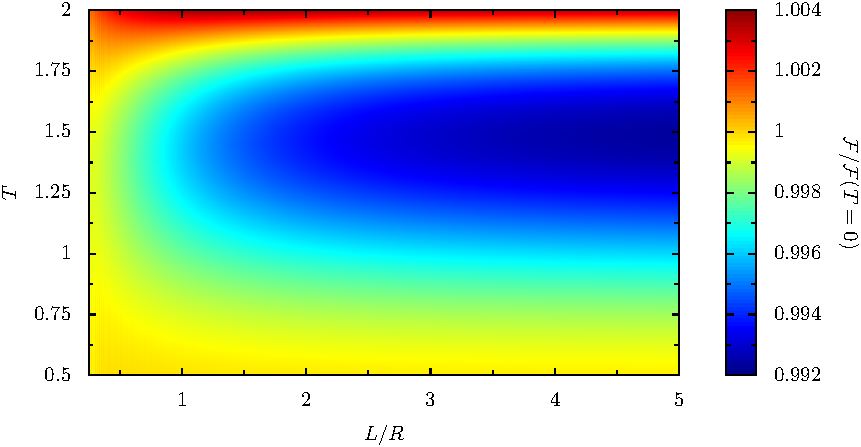
\includegraphics[scale=1]{plots/entropy_density_plot/plot_scaled_FbyF0.pdf}
    \end{center}

    \caption{$\mathcal{F}(T)/\mathcal{F}(T=0)$ in the range $0.25 \le L/R \le 5$ and $0.5 \le T \le 2$.}
    \label{fig:temp_intermediate}
\end{figure}

\begin{figure}
    \begin{center}
    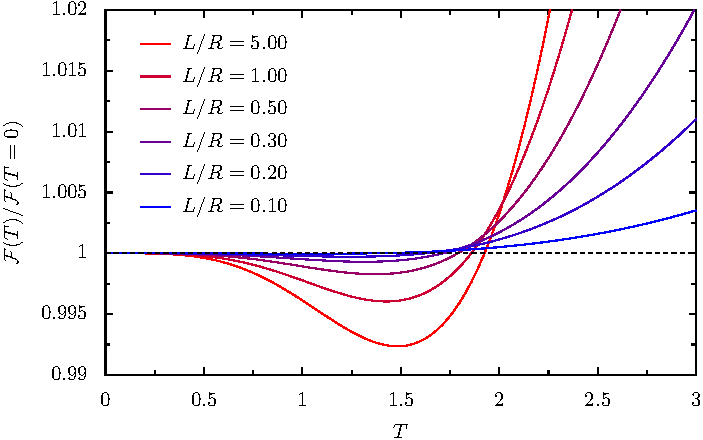
\includegraphics[scale=1]{plots/thermal/thermal.pdf}
    \end{center}

    \caption{$\mathcal{F}(T)/\mathcal{F}(T=0)$ for various separations dependent on temperature.}
    \label{fig:temp_intermediate2}
\end{figure}

For intermediate temperatures we have to rely on numerical results. In Fig.
\ref{fig:temp_intermediate} the ratio $\mathcal{F}(T)/\mathcal{F}(T=0)$ is
depicted in the range $0.25 \le L/R \le 5$ and $0.5 \le T \le 2$. In Fig.
\ref{fig:temp_intermediate2} we plot the ratio
$\mathcal{F}(T)/\mathcal{F}(T=0)$ for various separations $L/R$ dependent on
$T$. For a constant separation $L/R$ the ratio first decreases for increasing temperatures, reaches a minimum,
and increases afterwards. As the free energy is negative, a
minimum of the ratio $\mathcal{F}(T)/\mathcal{F}(T=0)$ corresponds to a maximum of the free energy and thus to
$S=0$. For large values of $L/R$ we find the large--distance limit: The
maximum of the free energy is located at $T\approx1.5$ in accordance with the
results of chapter \ref{chapter_ld}. For smaller separations the minimum is
reached at temperatures lower than $T\approx1.5$. We also see that the thermal increase of the
free energy is an effect in the order of per mille. Moreover, the effect becomes
more evident for large separations.

The numerical results were obtained using $\epsilon_p = 10^{-8}$, $\lmax =
\max{\left(20, \lfloor \eta \, R/L\rfloor\right)}$ with $\eta=6$. The
separations between two point is $\Delta_T \approx 0.0031$ and $\Delta_{L/R}
\approx 0.0045$.  The numerical data was converted using bilinear interpolation
to a resolution of 1000x1000 points in Fig. \ref{fig:temp_intermediate}.
